\documentclass[11pt,titlepage]{article}
\usepackage[reqno]{amsmath}
\usepackage{amssymb}
\usepackage{epsf}
\usepackage{epsfig}
\usepackage{url}

% === additional commands/packages/settings ===
\usepackage{graphicx,psfrag,natbib}
\usepackage{setspace}
\usepackage{vmargin}
\setpapersize{USletter}

% === dcolumn package ===
\usepackage{dcolumn}
\newcolumntype{.}{D{.}{.}{-1}}
\newcolumntype{d}[1]{D{.}{.}{#1}}

% === newcommands from sei.tex ===
\newcommand{\EI}{\ensuremath{{\mathfrak EI}}}
\newcommand{\Tiny}{\tiny}
\newcommand{\sump}{\sum_{i=1}^p}
\newcommand{\mean}{\frac{1}{p}\sump}
\newcommand{\ub}{\Dot{\beta}}
\newcommand{\ut}{\Dot{\theta}}
\newcommand{\bbeta}{{\mathfrak B}}
\newcommand{\btheta}{{\mathfrak T}}
\newcommand{\blambda}{{\mathfrak L}}
\newcommand{\bbetau}{\breve{\mathfrak B}}
\newcommand{\bV}{{\cal V}}
\newcommand{\sigmau}{\breve{\sigma}}
\newcommand{\Sigmau}{\breve{\Sigma}}
\newcommand{\rhou}{\breve{\rho}}
\newcommand{\psiu}{\breve{\psi}}
\newcommand{\Eu}{\breve{\text{E}}}
\newcommand{\Vu}{\breve{\text{V}}}
\newcommand{\Bb}{B^b}
\newcommand{\Bw}{B^w}
\newcommand{\NbD}{{N_i^{bD}}}
\newcommand{\NwD}{{N_i^{wD}}}
\newcommand{\NbR}{{N_i^{bR}}}
\newcommand{\NwR}{{N_i^{wR}}}
\newcommand{\NbN}{{N_i^{bN}}}
\newcommand{\NwN}{{N_i^{wN}}}
\newcommand{\tp}{{\mbox{\Tiny{+}}}}
\newcommand{\NpD}{{N_i^D}}
\newcommand{\NpR}{{N_i^{R}}}
\newcommand{\NpN}{{N_i^{N}}}
\newcommand{\Nbp}{{N_i^{b}}}
\newcommand{\Nwp}{{N_i^{w}}}
\newcommand{\Npp}{{N_i}}
\newcommand{\Nppp}{{N}}
\newcommand{\Nbpp}{{N^{b}}}
\newcommand{\Nwpp}{{N^{w}}}
\newcommand{\sumpN}{\sump\Npp}
\newcommand{\NsumpN}{\frac{1}{\Nppp}\sumpN}
\newcommand{\nbp}{{N_i^{bT}}}
\newcommand{\nwp}{{N_i^{wT}}}
\newcommand{\npp}{{N_i^{T}}}
\newcommand{\NbV}{{N_i^{bT}}}
\newcommand{\NwV}{{N_i^{wT}}}
\newcommand{\NpV}{{N_i^{T}}}
\newcommand{\xb}{\bar{X}}
\newcommand{\wb}{\bar{W}}
\newcommand{\tb}{\bar{T}}
\newcommand{\cx}{{\mathbb X}}
\newcommand{\cw}{{\mathbb W}}
\newcommand{\ct}{{\mathbb T}}
\newcommand{\cpij}{{\mathbb P}^*_{ij}}
\newcommand{\cpi}{{\mathbb P}^*_i}
\newcommand{\cwd}{{\dot{\mathbb W}}}
\newcommand{\ctd}{{\dot{\mathbb T}}}
\newcommand{\cxd}{{\dot{\mathbb X}}}
\newcommand{\cxb}{\bar{\mathbb X}}
\newcommand{\cz}{{\mathbb G}}
\newcommand{\ch}{{\mathbb H}}
\newcommand{\cm}{{\mathbb M}}
\newcommand{\E}{{\textbf{E}}}
\newcommand{\V}{{\textbf{V}}}
\newcommand{\C}{{\textbf{C}}}
\newcommand{\rE}{{\text{E}}}
\newcommand{\rV}{{\text{V}}}
\newcommand{\rC}{{\text{C}}}
\newcommand{\TN}{\text{TN}}
\newcommand{\BN}{\text{BN}}
\newcommand{\N}{\text{N}}
\renewcommand{\P}{\text{P}}
\newcommand{\D}{\textbf{D}}
\newcommand{\R}{\ensuremath{\textbf{R}}}
\newcommand{\Rr}{\ensuremath{\{\textbf{R}\diagdown r}\}}
\newcommand{\bC}{\ensuremath{\textbf{C}}}
\newcommand{\Cc}{\ensuremath{\{\textbf{C}\diagdown c}\}}
\newcommand{\one}{{\mathbf{1}}}
\newcommand{\Q}{\ensuremath{\overset{\vspace{3em}}{\text{\Huge ?}}}}
\newlength{\padsp}
\settowidth{\padsp}{$(\beta^w_i=\nwp/\Nwp)$}
\newcommand{\padbw}{\hspace*\padsp}
\newcommand{\bkappa}{\boldsymbol{\kappa}}

\newcommand{\bb}{\beta^{\text{bad}}}
\newcommand{\bg}{\beta^{\text{good}}}
\renewcommand{\bibitem}{\vskip 2pt\par\hangindent\parindent\hskip-\parindent}

\title{Analyzing Second-Stage Ecological Regressions:\\
  Extensions to Herron and Shotts}

\author{Christopher Adolph\thanks{Ph.D. candidate, Department of
    Government, Harvard University. (Littauer Center---North Yard,
    Harvard University, Cambridge MA 02138;
    \texttt{http://chris.adolph.name},
    \texttt{cadolph@Fas.Harvard.Edu}).}
\and %
Gary King\thanks{Professor of Government, Harvard University and
  Senior Science Advisor, World Health Organization (Center for Basic
  Research in the Social Sciences, 34 Kirkland Street, Harvard
  University, Cambridge MA 02138; \texttt{http://GKing.Harvard.Edu},
  \texttt{King@Harvard.Edu}, (617) 495-2027).}  }

\begin{document}
\maketitle
% \begin{abstract}
%   Herron and Shotts make an important contribution by 
%   noting that the interesting point that 
%   the only time the fully adjusted procedure clearly dominates least
%   squares regression is when the bounds are uninformative and
%   ecological inference is so risky that, unless additional information
%   was available, no analysis should be trusted at all.
% \end{abstract}

\section{Introduction}

We take this opportunity to comment on Herron and Schotts' article
(hereinafter HS) because of its potential to affect the way a
considerable body of practical research is conducted, and because of
HS's interesting and productive ideas.  HS's paper is based on the
suggestions in three paragraphs in King (1997: 289--90).  Since these
paragraphs were not summarized in HS, we thought they might be a
useful place to start:
\begin{quotation}
  If a second stage analysis is conducted, least squares regression
  should probably not be used in most cases, even though it may not be
  particularly misleading.  The best first approach is usually to
  display a scatterplot of the explanatory variable (or variables)
  horizontally and (say) an estimate of $\beta_i^b$ or $\beta_i^w$
  vertically.  In many cases, this plot will be sufficient evidence to
  complete the second stage analysis.
  
  If it proves useful to have more of a formal statistical approach,
  and many of the actual values of $\beta_i^b$ fall near zero or one,
  then some method should be used that takes this into account.  The
  data could be transformed, via a logit or probit transformation, or
  [the ``extended model''] could be applied\ldots.  Whatever method is
  chosen, the researcher should be careful to include the fact that
  some estimates of $\beta_i^b$ are more uncertain than others.
    
  In practice, a weighted least squares linear regression may be
  sufficient in many applications, with weights based on the standard
  error of $\beta_i^b$ (or other quantity of interest).  Researchers
  should be careful in applying this simplified method here, and
  should verify its assumptions with scatterplots. \ldots This is not
  as theoretically elegant a procedure as the more formal set up in
  [the ``extended model''] but it is simple, relatively robust, and
  probably complete enough to be of use in many applications.
\end{quotation}  

HS add to the ideas in these paragraphs by pointing out that
precinct-level estimates from EI regress to the mean.  This
``shrinkage'' property is indeed a characteristic of EI, as it is for
all Bayesian models (of which EI is one).  Shrinkage results in
optimal estimates, that is with the smallest possible mean square
error.  Thus, we agree with the implication of HS's article that the
best possible estimate of $\beta^b_i$, under HS's assumptions, is that
produced by EI.  But HS also make the interesting and correct point
that using Bayesian mean posterior estimates with this property, like
those given by EI, as dependent variables in least squares regression
can, under some circumstances, produce biased estimates.  This central
point of HS's paper is an important contribution and one on which we
build here.

Instead of least squares regression, HS's suggested procedure is to
use a bias adjusted slope for the second stage regression but to leave
the constant term unchanged.  Their adjustment is based on linear
approximations within the classical linear econometric theory
framework.  The problems with identify with HS's approach are due to
assuming linearity when modeling an inherently nonlinear and bounded
relationship (i.e., their methods by definition misses the information
in the bounds), not completing the task they set for themselves within
this framework, and never actually computing the correction they
propose in any of their simulations.  The primary advance of EI is in
resolving the longstanding debate between supporters of Goodman's
(1959) unbounded linear regression approach and Duncan-Davis' (1953)
method of bounds, by incorporating all information in both into the
same model.  HS fall back to Goodman's unbounded approach and so miss
the highly informative deterministic information in the aggregate
data.

We replicated HS's simulations without trouble.  We then examined how
well their adjusted regression procedure fit the observed data based
on the estimated $\hat\beta_i^b$ and the true (normally unobserved)
$\beta_i^b$.  We find that correcting the slope but not the constant,
as HS suggest, is considerably worse than an unadjusted regression of
$\hat\beta_i^b$ on $Z$ and every other procedure discussed in HS's
paper and the literature we have examined.  This is true even if we
knew the true value of the adjustment.  The regression line from HS's
method usually misses the cloud of true $\beta_i^b$ points by a wide
margin.

We therefore begin by extending HS's partial adjustment procedure,
within their linear econometric framework, by developing an adjustment
for the constant term also.  This fully adjusted second stage
regression method naturally extends HS's framework and dominates HS's
procedure.  We also compare our fully adjusted procedure to unadjusted
linear regression and find four prototypical situations likely to
arise in practice.  Since each situation is easily detectable from the
available aggregate data, users will know which situation they are in
and can take the appropriate action.  As it turns out, the HS
partially adjusted procedure is never called for.  Overall, when the
bounds are narrow, the fully adjusted procedure can be computed, but
the adjustment makes little difference.  When the bounds are wide, the
true adjustment factor could make a big difference but the adjustment
cannot be reliably estimated, and so the procedure cannot be applied.
Thus, in the first prototypical case, when the bounds are very wide,
making any ecological inferences at all in the first stage is
inadvisable (unless one has strong auxiliary information), due to
extreme model dependence; and in this situation the correction will
not help.  In the other three situations, the best procedures are
unadjusted least squares, unadjusted weighted least squares
regression, and a logistic regression procedure, respectively.  (The
only situation when the adjustment will lead to improvements is with
wide bounds and the true value of the adjustment is known, which
describes HS's simulation techniques but not any real application.)

\section{A Fully Adjusted Second Stage Regression Model}
\label{s:fulladj}

We simplify HS's notation where possible and present our fully
adjusted method with their adjustment as a special case.\footnote{Our
  notation deviates from HS only to ensure logical consistency, which
  is not always present in the original.  For example, their Equations
  (7) and (8) have different dependent variables, $\beta_i^b$ and
  $\hat\beta_i^b$ set equal to the same entire right side of the
  equation in both cases ($\alpha+\gamma'Z_i+\nu_i$).  Later in their
  paper, they allow $\gamma$ to differ between the two (calling the
  first $\gamma_R$ and the second $\gamma_U$), but do not fix the
  constant term (or error terms).  We fix these issues and others,
  since what they intended can be ascertained.}

First, let the expectation of $\beta_i^b$ conditional on $Z_i$ be
approximated by
\begin{equation}
  \label{true}
  E(\beta_i^b)=\alpha_R+\gamma_R Z_i,
\end{equation}
so that estimates of $\alpha_R$ and $\gamma_R$ are the immediate goal
of the analysis.  Also let the expectation of $\hat\beta_i^b$
conditional on $Z_i$ be
\begin{equation}
  \label{est}
  E(\hat\beta_i^b)=\alpha_U+\gamma_U Z_i,
\end{equation}
which is of course well estimated by least squares.  HS then assume
that the error in estimating $\hat\beta_i^b$ by EI is a linear
function of $\beta_i^b$:
\begin{equation}
  \label{hserr}
  E(\hat\beta_i^b - \beta_i^b) = \delta_0^b + \delta_1^b\beta_i^b.
\end{equation}
Then solving (\ref{hserr}) for $E(\hat\beta_i^b)$ and substituting the
result into (\ref{est}) gives a more informative version of (\ref{true}):
\begin{equation}
  \label{adj}
  E(\beta_i^b) = \left(\frac{\alpha_U-\delta_0^b}{1+\delta_1^b}\right)
  + \left(\frac{\gamma_U}{1+\delta_1^b}\right)Z_i.
\end{equation}
Thus, we know that the quantities of interest, $\alpha_R$ and
$\gamma_R$, can be expressed as the intercept and slope of
(\ref{adj}).  If we can estimate the components of each, we can derive
a consistent estimator, assuming HS's linearity and unboundedness
assumptions are not too far off.

\section{Correcting and Extending Herron and Shotts' Estimation
  Procedure}

HS offer an estimation algorithm for correcting the slope term in
their Section 7.2.  This procedure is intuitive and we can easily
generalize it to provide a correction for the intercept as well.
Unfortunately, the procedure itself is flawed for two reasons.  First,
it conditions on the point estimate for $\breve\psi$, and thus assumes
the absence of estimation uncertainty.  Ignoring uncertainty would
bias standard errors and confidence intervals, of course, but HS do
not calculate these.  However, since their estimation procedure is
nonlinear (due to the ratios in (\ref{adj})), ignoring estimation
uncertainty also affects their point estimates in finite samples.  And
second, the procedure calls for drawing only a single simulation of
$(\beta_i^b,\beta_i^w)$ for each observation.  As a result, the
estimate includes substantial Monte Carlo approximation error.  The
error can be eliminated by running their entire procedure many times
and averaging.  Although fixing these problems would not have
substantially changed the estimates presented in their paper, they
will matter in some applications.  We therefore develop and use an
estimation algorithm that corrects these problems, a nice side effect
of which is the ability to compute standard errors and confidence
intervals, which were not available in HS's version.\footnote{To
  define our estimation algorithm, let a symbol with a tilde on it
  denote a value of that quantity randomly drawn from its posterior
  density.  To implement our procedure for a given $X$ and $T$: (1)
  run EI on $X$ and $T$; (2) draw $\tilde\psiu$ from its posterior
  provided by EI; (3) take $p$ draws of
  $(\tilde\beta_i^b,\tilde\beta_i^w)$ from a truncated normal density
  with parameter vector $\tilde\psiu$, (4) compute a new $T_i$ as
  $\tilde T_i=\tilde\beta_i^bX_i+\tilde\beta_i^w(1-X_i)$; (5) run EI
  on $X_i$ and $\tilde T_i$ to yield estimates
  ($\hat\beta_i^b,\hat\beta_i^w$) for all $i$; (6) regress
  ($\hat\beta_i^b-\beta_i^b$) on $\beta_i^b$ to estimate
  $\delta_0^b$ and $\delta_1^b$; (7) regress $\hat\beta_i^b$ on $Z_i$
  yielding the estimated intercept $\hat\alpha_U$ and slope
  $\hat\gamma_U$; (8) compute the adjusted intercept as
  $(\hat\alpha_U-\hat\delta_0^b)/(1+\hat\delta_1^b)$ and adjusted
  slope as $\hat\gamma_U/(1+\hat\delta_1^b)$; (9) repeat steps (2)-(8)
  a sufficient number of times to eliminate Monte Carlo approximation
  error; (10) and average the simulations in (9) to get point
  estimates, take their standard deviation for standard errors, or
  sort them and use percentile values for confidence intervals.}

\section{Herron and Shotts' Monte Carlo Simulations}

The Monte Carlo procedure used to generate results by HS is
inappropriate to the task of evaluating second stage regressions.  HS
draw $\beta_i^b$ from the EI model without covariates.  Then they
create the covariate for the second stage $Z_i$ endogenously as equal
to $\beta_i^b$ plus random noise.  The problem with this procedure is
that it induces immense attenuation bias due to random measurement
error in the explanatory variable, quite apart from any attenuation
bias that may occur due to the Bayesian shrinkage error in the EI
estimate.

This problem can be seen by studying the parameters of the model they
created from which to draw their Monte Carlo data.  In this model, the
slope of the coefficient on the covariate in the second stage
regression is 1 (in their notation, $\gamma_R=1$).\footnote{Under the
  HS Monte Carlo setup, $E(\beta_i^b)=\alpha_R+\gamma_R Z_i$, where
  $Z_i=\beta_i^b+\tau_i$ and $E(\tau_i)=0$.  Hence
  $E(\beta_i^b)=\alpha_R+\gamma_RE(\beta_i^b+\tau_i)=\alpha_R+\gamma_R\beta_i^b$.
  which implies that $\alpha_R=0$ and $\gamma_R=1$.}  However, the
estimates of this slope from their simulations of the \emph{true}
$\beta_i^b$ (i.e., without any attenuation bias in the dependent
variable at all) regressed on $Z$ gives a drastically biased estimate.
This slope estimate does not appear in their article, but we were able
to to replicate their Table 2 exactly, and in our Table \ref{t:hsrep}
present these numbers.  As can be seen, whereas the theoretical value
of $\gamma_R$ is 1 in each case, their estimates indicate that
$\hat\gamma_R\approx 0.07$.  Thus, since the unadjusted method is
unable to recover the coefficients without shrinkage when using the
true value of the dependent variable, this Monte Carlo setup is
inappropriate for assessing a dependent variable that is estimated.
\begin{table}[tb]
\label{t:hsrep}
\begin{center}
\begin{tabular}{cc|c c c}
Model Parameters & Truth & \multicolumn{3}{c}{HS Estimates} \\
$\breve\psi$  & $\gamma_R$ & $\hat\gamma_R$  &       $\hat\gamma_U$ & $\hat\gamma_A$ \\\hline
(0.5, 0.5, 0.1, 0.1, 0)&1 &       0.04    &       0.02    &       0.04        \\
(0.75, 0.5, 0.1, 0.1, 0) &1       &       0.04    &       0.02    &       0.04        \\
(0.75, 0.75, 0.1, 0.1, 0) &1      &       0.04    &       0.02    &       0.04     \\
(0.9, 0.9, 0.1, 0.1, 0) &1&       0.02    &       0.01    &       0.02          \\
(0.5, 0.5, 0.32, 0.1, 0) &1       &       0.19    &       0.13    &       0.19        \\
(0.6, 0.6, 0.1, 0.32, 0) &1       &       0.04    &       0.01    &       0.04     \\
(0.9, 0.1, 0.32, 0.32, 0)&1       &       0.15    &       0.08    &       0.15        \\
(0.5, 0.5, 0.1, 0.1, 0.3)&1       &       0.04    &       0.02    &       0.04     \\
\hline
\end{tabular}
\end{center}
\caption{\em Estimated and ``true'' slopes from 
second-stage regressions based on Herron and Schott's Monte Carlo 
procedure. This table replicates the results of simulations presented in
HS Table 2.  All results are averages over 100 simulations.  
The difference and ratios presented in HS Table 2 were  
successfully replicated, and are not shown here.}
\end{table}

A second problem with the Monte Carlo procedure employed by HS is that
it artificially rules out nonlinear relationships between $\beta_i^b$
and $Z_i$ created by the bounds.  By constructing their explanatory
variable, $Z_i$, from the bounded $beta_i^b$'s (plus a normal
disturbance), they artificially restrict the relationship between the
two to be linear and to always be contained within the [0,1] bound on
$beta_i^b$.  Within this framework, testing the robustness of the HS
adjustment to the sort of nonlinear relationships which may crop up in
applied research is impossible.

\section{An Improved Monte Carlo Simulation} \label{s:alt}

Most of our conclusions below do not depend on changing the simulation
method, but we do so in order to make the results more coherent.  To
simulate, we follow the logic of the extended EI model.  Thus, we
first fix $X$, the covariates $Z$ (to values uncorrelated with $X$),
the values for the intercept and the slope parameter on $Z_i$, and the
variance and covariance parameters of the truncated bivariate normal.
Then, for each simulation, we draw the $\beta_i^b$'s from the extended
EI model conditional on $X_i$ and $Z_i$ (without mean centering).  The
assumption that $X_i$ and $Z_i$ are uncorrelated enables us to run a
(first-stage) basic EI model (i.e., with no covariates) without
inducing aggregation bias.  (The assumption is of course less
important when the bounds are more informative, but we retain it for
simplicity in the simulations below.)  With this setup, unless the
relationship is clearly nonlinear because the bounds are very
influential, a regression of the true $\beta_i^b$ on $Z_i$ recovers
the intercept and slope coefficients accurately.

We use this Monte Carlo setup to illustrate four prototypical
situations that in our experience maps out the space of applications
in which the various methods work in different ways.  (That is, all
the simulations we have run look like these plots or roughly speaking
convex combinations of them.)

First, when ecological data have very wide bounds, EI (and any method
of ecological inference) will be sensitive to modeling assumptions,
(the problem inherent in the original Goodman's regression no matter
what the data looked like).  In many applications with data like
these, no ecological inference should be conducted unless one has some
special auxiliary information about the model assumptions.  If one
proceeds to the second stage anyway then, since shrinkage probably
exists in the $\beta_i^b$'s, the true (unobserved) value of the full
adjustment would make for an improvement over least squares on the
estimated $\hat\beta_i^b$'s.  Of course, the true adjustment is not
known and needs to be estimated.  Unfortunately, it cannot.  The
reason is that EI models $\beta_i^b$ as a random effect constrained to
be within the precinct-level bounds.  If $Z_i$ is not in the EI first
stage (which is true by definition, since if it were included we
wouldn't need a second stage), then the \emph{only} information in
$\hat\beta_i^b$ that could be predicted by $Z_i$ would come from the
bounds.  The same is true of the adjustment procedure: the \emph{only}
information with which to estimate $\delta_0$ and $\delta_1$ comes
from the bounds.  If the bounds are relatively uninformative, as we
are assuming in this first prototypical case, then there is little
information with which to estimate the adjustment.  On reflection,
this should not be a surprise: an unbounded random effect variable
must be unrelated to all measured variables except by chance.

Figure \ref{f:wide} plots the covariate $Z_i$ horizontally by the true
$\beta_i^b$ (in the left graph) and the estimated $\hat\beta_i^b$ (in
the right graph) vertically.  Note how the unadjusted least squares
line (marked LS) fits the estimated points well (in the right graph)
but are attenuated for the true points (in the left).  Since the
bounds are all very wide, the variances are almost constant and so the
weighted least squares (marked WLS) line is practically on top of the
LS line.  The line representing the fully adjusted method using the
\emph{true} values of $\delta_0$ and $\delta_1$ (true adjustment is
marked TA) fits the true points well, and would correct for the
attenuation.  The actual fully adjusted method (marked FA) as
estimated from the data also appears, but due to the wide bounds it is
not a good estimate and is worse than LS and WLS.  Figure \ref{f:wide}
also plots Herron and Shotts' partially adjusted method (marked HS),
which is more biased than any of the alternatives, a problem which
grows in severity as the mean of $Z$ departs from zero.  Since HS's
proposal is never better than full adjustment, and often dramatically
worse, we do not consider it further.
\begin{figure}[t]
  \begin{center}
    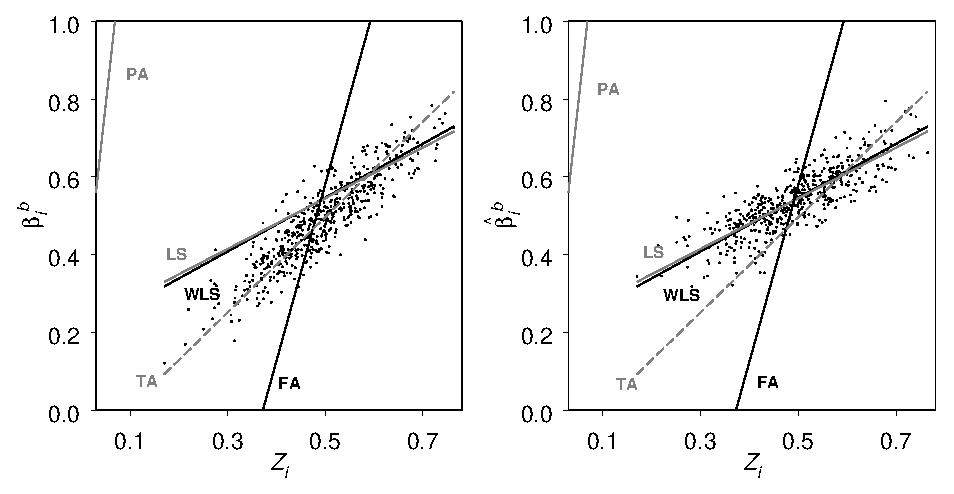
\epsfig{file=wide.eps}
    \caption{Data with Wide Bounds. Plot of $Z_i$ horizontally by
      the estimated $\hat\beta_i^b$ vertically (in the right graph)
      and the true $\beta_i^b$ (in the left graph), with fits for
      Herron and Shotts' partially adjusted procedure (HS), least
      squares (LS) and weighted least squares (WLS) almost on top of
      one another, our fully adjusted method (FA), and the full
      adjustment based on the true values of $\delta_0$ and $\delta_1$
      (TA).  Clearly TA fits the true points best, but is
      unfortunately badly estimated by FA.  Data were generated from
      the extended EI model with $X \sim \textrm{Uniform}(0,0.2)$, $Z
      \sim \textrm{Normal}(0.5,0.1)$, $\breve\bbeta_i^b = [-2 \times
      (\sigmau_b^2 + 0.25) + 0.5] + Z_i$, $\breve\bbeta_i^w = [-2
      \times (\sigmau_w^2 + 0.25) + 0.5] + Z_i$, $\sigmau_b = 0.05$,
      $\sigmau_w = 0.05$, and $\rhou = 0$.}
    \label{f:wide}
  \end{center}
\end{figure}

Second, when the bounds are at least somewhat informative (that is,
when few of the bounds are extremely wide), we are in the situation
when we would be more likely to trust ecological inferences using EI
(or another method that takes into account the information in the
precinct-level bounds).  When the relationship is approximately (or
locally) linear, we find that ordinary least squares regression
usually does as well as, and often better than, the fully adjusted
procedure.  Figure \ref{f:narrow} gives one example where least
squares, weighted least squares, and our fully adjusted method all
give approximately the same estimates.
\begin{figure}[t]
  \begin{center}
    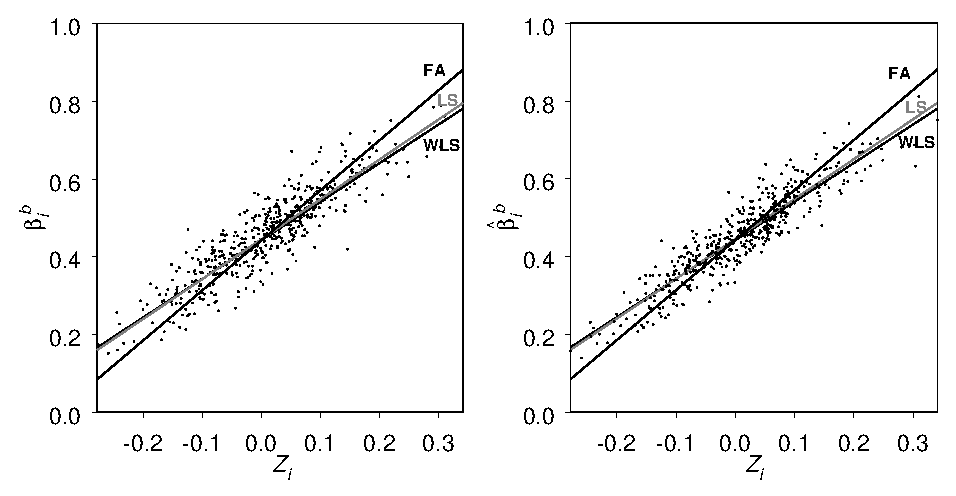
\epsfig{file=narrow.eps}
    \caption{Data with Informative Bounds. Plot of the $Z_i$ horizontally by
      the estimated $\hat\beta_i^b$ vertically (in the right graph)
      and the true $\beta_i^b$ (in the left graph) with fits for least
      squares (LS) and weighted least squares (WLS) appears almost on
      top of one another, and our fully adjusted method (FA).  Note
      how all three methods give almost the same answer. Data were
      generated from the extended EI model, with $X \sim
      \textrm{Uniform}(0.2,1)$, $Z \sim \textrm{Normal}(0,0.1)$,
      $\breve\bbeta_i^b = [-0.2 \times (\sigmau_b^2 + 0.25) + 0.5] +
      Z_i$, $\breve\bbeta_i^w = [0.6 \times (\sigmau_w^2 + 0.25) +
      0.5] + Z_i$, $\sigmau_b = 0.05$, $\sigmau_w = 0.05$, and
      $\rhou = 0$.}
    \label{f:narrow}
  \end{center}
\end{figure}

Third, when some observations have wide bounds and others have narrow
bounds, and $\hat\beta_i^b$ is an approximate (or locally) linear
function of $Z_i$, (unadjusted) weighted least squares regression will
often be substantially less biased than least squares, and be
approximately equivalent to or better than the fully adjusted
procedure.\footnote{Like all weighted regressions, this procedure
  would have higher variance than LS. HS studied consistency, and
  implicitly bias, but did not address other properties, such as
  efficiency.  A complete evaluation would of course consider these
  properties as well.}  This is contrary to HS's claims that WLS would
not make a difference; what they missed by applying a linear
regression framework to this problem with bounds and nonlinearity is
that the degree of attenuation is greater when the bounds are wider
--- as can be seen by the differences between Figures \ref{f:wide} and
\ref{f:narrow} --- and so the weights are correlated with the
attenuation bias and can at least partially adjust for it.  Figure
\ref{f:mixed} provides an example of this phenomenon.  We generated
the data for this figure from the same model as the other figures,
changing only the parameter values so that the points were affected by
the bounds.  The effect of the wide bounds on some observations can be
seen by the attenuation in the set of points forming a flatter slope
in the right graph (as compared to the left graph which has no such
feature).  As a result, the least squares (LS) line is a good deal
flatter than it should be (as judged by the fit to the points in the
left graph) but the (unadjusted) weighted least squares (WLS) line
corrects for most of the attenuation.  The fully adjusted (FA) line is
badly estimated and misses the mark.
\begin{figure}[t]
  \begin{center}
    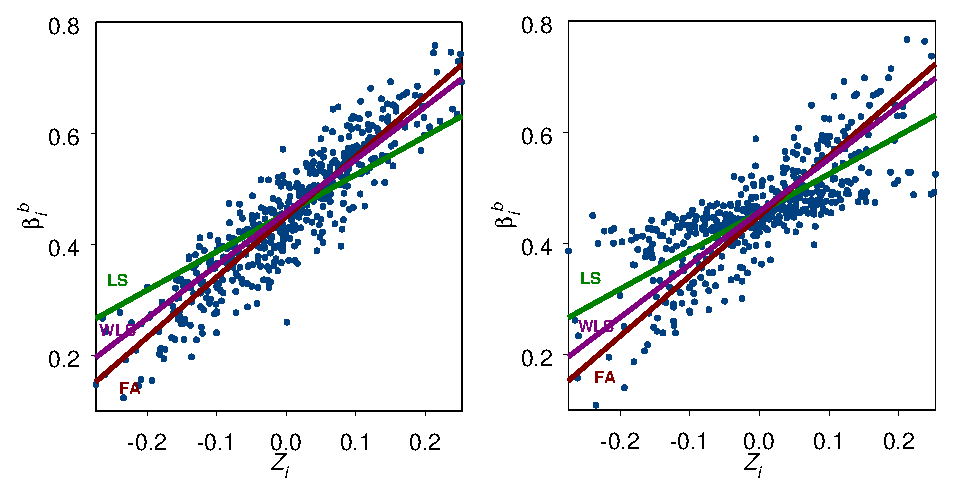
\epsfig{file=mixed.eps}
    \caption{Data with Narrow and Wide Bounds. Plot of the $Z_i$ 
      horizontally by the estimated $\hat\beta_i^b$ vertically (in the
      right graph) and the true $\beta_i^b$ (in the left graph) with
      fits for least squares (LS), weighted least squares (WLS), and
      our fully adjusted method (FA).  Note how (unadjusted) WLS
      corrects for most of the attenuation bias.  Data were generated
      from the extended EI model, with $X \sim
      \textrm{Uniform}(0.2,1)$ and $(0.8,1)$, $Z \sim
      \textrm{Normal}(0,0.1)$, $\breve\bbeta_i^b = [-0.2 \times
      (\sigmau_b^2 + 0.25) + 0.5] + Z_i$, $\breve\bbeta_i^w = [0.6
      \times (\sigmau_w^2 + 0.25) + 0.5] + Z_i$, $\sigmau_b = 0.05$,
      $\sigmau_w = 0.05$, and $\rhou = 0$.}
    \label{f:mixed}
  \end{center}
\end{figure}

Finally, when the relationship is nonlinear, as is often observably
the case because of the bounds, then any (adjusted or unadjusted)
linear second stage procedure can produce impossible results.  In this
situation, a scatterplot or an appropriate nonlinear procedure would
be better.  The fully adjusted procedure in this situation often
produces more out of bounds predictions than the unadjusted procedure.
(In this case, WLS is also inappropriate, both because the assumption
of linearity does not hold, and because $\hat\beta_i^b$'s at the
extremes have standard errors of zero or nearly so.  Giving extra
weight to these observations tends to bias the estimate of the slope
downwards.)  Figure \ref{f:nonlinear} illustrates these issues.  In
this example, we also include a nonlinear model by regressing a logit
transformation of $\hat\beta_i^b$,
$\ln(\hat\beta_i^b/(1-\hat\beta_i^b))$, on $Z_i$ and using simulation
to compute the regression line.  This line (marked LT) clearly gives a
far better fit than any of the other methods.  It is also the only
method that does not extend above 1 or below 0 for $\beta_i^b$ (i.e.,
into the impossible region) for some values of $Z_i$.
\begin{figure}[t]
  \begin{center}
    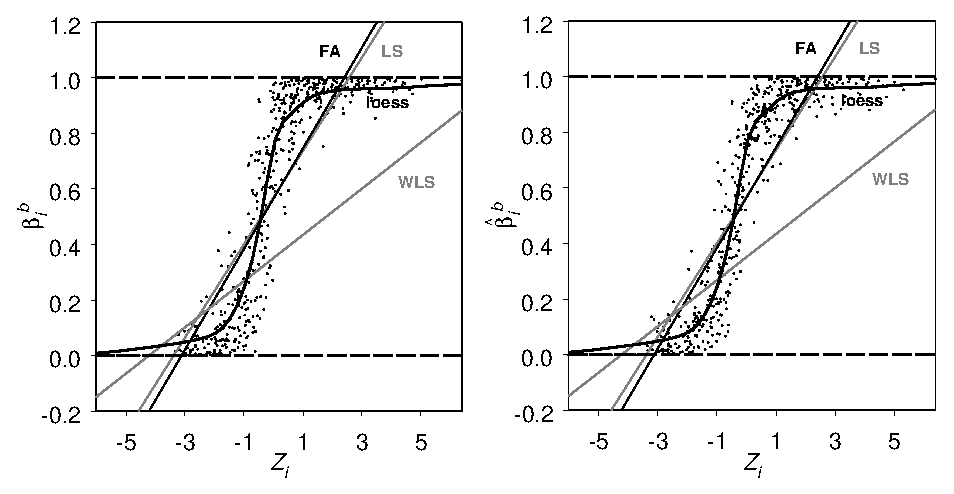
\epsfig{file=nonlinear.eps}
    \caption{Data with a Nonlinear Relationship.  Plot of $Z_i$ 
      horizontally by the estimated $\hat\beta_i^b$ vertically (in the
      right graph) and the true $\beta_i^b$ (in the left graph) with
      fits for least squares (LS) and our fully adjusted method (FA)
      almost on top of one another, weighted least squares (WLS), and
      the better fitting logistic transformation (LT).  Note how all
      the linear methods give out of bounds predictions.  Data were
      generated from the extended EI model, with $X \sim
      \textrm{Uniform}(0,1)$, $Z \sim \textrm{Normal}(0,2)$,
      $\breve\bbeta_i^b = [1.2 \times (\sigmau_b^2 + 0.25) + 0.5] +
      Z_i$, $\breve\bbeta_i^w = [1.2 \times (\sigmau_w^2 + 0.25) +
      0.5] + Z_i$, $\sigmau_b = 0.3$, $\sigmau_w = 0.3$, and
      $\rhou = 0$.}
    \label{f:nonlinear}
  \end{center}
\end{figure}

\section{Adjustments in Practice: A Replication of Burden and Kimball (1998)}

At least in some applications, differences among the various methods
of second stage analysis make little difference.  We replicate Burden
and Kimball's (1998) study of split-ticket voting, the empirical study
HS focus the most, and find that none of the proposed corrections
affect the substantive conclusions of the original study.  Table
\ref{t:bkrep} presents these results (assuming arguendo that other
features of their model are correctly specified).
\begin{table}[th]
\label{t:bkrep}
\begin{center}
\begin{tabular}{lcccccc}
& \multicolumn{3}{c}{\underbar{President/House}} & \multicolumn{3}{c}{\underbar{President/Senate}}\\
Variable        &       LS      &       FA      &       WLS     &       LS      &       FA      &       WLS     \\
\hline
Spending ratio  &       0.350   &       0.446   &       0.471   &       0.318   &       0.441   &       0.426   \\
        &       (0.021) &       (0.193) &       (0.032) &       (0.094) &       (0.174) &       (0.111) \\
Ideological distance    &       -       &       -       &       -       &       -0.025  &       -0.035  &       -0.053  \\
        &               &               &               &       (0.040)  &       (0.014) &       (0.051) \\
Democratic incumbent    &       0.106   &       0.135   &       0.090   &       0.059   &       0.081   &       0.028   \\
        &       (0.015) &       (0.056) &       (0.025) &       (0.052) &       (0.032) &       (0.063) \\
Ballot format   &       -0.032  &       -0.041  &       -0.074  &       -0.050  &       -0.070  &       -0.062  \\
        &       (0.008) &       (0.018) &       (0.011) &       (0.037) &       (0.028) &       (0.047) \\
South   &       0.041   &       0.053   &       0.081   &       0.046   &       0.064   &       0.003   \\
        &       (0.009) &       (0.023) &       (0.011) &       (0.052) &       (0.025) &       (0.058) \\
Constant        &       0.067   &       -0.181  &       0.051   &       0.144   &       -0.159  &       0.168   \\
        &       (0.008) &       (0.507) &       (0.011) &       (0.084) &       (0.422) &       (0.102) \\
$N$     &       361     &       361     &       361     &       32      &       32      &       32      \\
\hline
\end{tabular}
\end{center}
\caption{\em Replication of Burden and Kimball (1998: Table 6).  
The dependent variable is the estimated proportion of 
voters who split their tickets between the Republican presidential 
candidate and a Democratic Congressional candidate in the 1988 general 
election, obtained from EI.  LS denotes least squares estimates, FA 
full adjustment, and WLS weighted least squares.  Standard errors in 
parentheses.}
\end{table}

Burden and Kimball investigated ticket-splitting behavior in the 1988
U.S. general election.  They used EI to estimate the proportion of
Bush voters who also voted for a Democratic Congressional candidate
(considering House and Senate separately), then employed these
estimates as dependent variables in second-stage regressions.  Their
goal was to show whether ticket splitting was the result of
intentional efforts by moderate voters to balance ideologically
disparate candidates (Alesina and Rosenthal, 1995) or an artifact of
differing campaign resources (Jacobson, 1997) and ballot formats
(Beck, 1997).  They found that the degree of ticket splitting falls
with the ideological distance between presidential and Senate
candidates, undermining the balancing thesis, but also that
differences in campaign resources appear to predict ticket splitting
quite well.

Burden and Kimball's work is consistent with our recommendations.  The
relationship they examine is approximately linear, and few of the
bounds are particularly wide or narrow.  Appropriately, they report
both least squares and weighted least squares estimates, which we were
able to replicate reasonably well (see columns LS and WLS in Table
\ref{t:bkrep}).  We also computed our fully adjusted method (column
FA).\footnote{Burden and Kimball estimate their dependent variable
  using a two-stage EI procedure for a $2\times 3$ table.  We used
  only the second stage to compute the fully adjusted method.} In most
cases, the FA results are comparable to, or bracketed by, the LS and
WLS estimates (which Burden and Kimball considered sufficiently
similar to use interchangeably).  In particular, we obtain generally
similar results for the two most important variables in Burden and
Kimball's model, spending ratio and ideological distance.  All three
methods thus support Burden and Kimball's argument that
ticket-splitting results not from intentional balancing, but as an
unintentional result of campaign specific factors.

\section{Concluding Suggestions}

As suggested in King (1997) and quoted above, ``The best first
approach is usually to display a scatterplot of the explanatory
variable (or variables) horizontally and (say) an estimate of
$\beta_i^b$ or $\beta_i^w$ vertically.  In many cases, this plot will
be sufficient evidence to complete the second stage analysis.''  This
approach remains accurate.  Indeed \emph{show us the data} is a good
general motto for any statistical analysis, especially those with
complex nonlinear and bounded variables such as those resulting from
making ecological inferences.  To this scatterplot, we would suggest
adding information on the bounds.  This can be done by adding a thin
vertical line representing the bounds on $\beta_i^b$ for each
$(\hat\beta_i^b,Z_i)$ point plotted (e.g., King, 1997: Figure 13.2).
From this figure, we can then see all the information in the data,
precisely how informative the bounds are, and whether the bounds are
of constant or variable width.

For researchers who wish a simple approximation to estimating a second
stage relationship, the information provided in this article should
provide a guide to helping choose intelligently among the unadjusted,
adjusted, weighted, or nonlinear methods.  Researchers can easily tell
in which of the four prototypical situations listed and illustrated in
Section \ref{s:alt} their data fall, and they can take the action
indicated.

If a more formal statistical approach seems desirable, then a good
method must go beyond classical linear econometric theory.  It must
take into account (a) the nonlinear nature of the problem, (b) the
bounded nature of the second stage dependent variable with the width
of the bounds varying over observations, (c) the heteroskedasticity,
and (d) the effect of any possible logical inconsistency of the first
and second stages of the analysis (since two-step statistical methods
need not be logically consistent to work well; see, e.g., Meng, 1994).
At present, the only model that has been proposed with all these
properties is the extended EI model that allows covariates to be
included as part of the EI estimation procedure (King, 1997: Ch.9).
HS are correct that this extended model is sometimes only weakly
identified, but that is only when the bounds are not narrow enough and
$X$ is included among the covariates or highly related to $Z$.  In
other cases, with narrow bounds or even wide ones when $Z$ is
unrelated to $X$, the extended model can be strongly identified and so
can be used in many cases without problem.  Imai and King (2002)
demonstrate how to compute first differences and other quantities of
interest from the extended EI model, and they report on extensions of
the EI software to make this easy to apply.

Econometric theory and the classical linear regression framework works
well for what it was designed for.  However, in models with nonlinear
relationships or sample spaces or parameter spaces that are highly and
differentially bounded, such as in ecological inference problems,
political methodologists need to look elsewhere or develop their own
methods.  

HS have made an important contribution by highlighting what turns out
to be the shrinkage property of Bayesian point estimates like those
provided by EI.  We are in their debt for pointing this out and
stimulating the ideas and discussions offered herein.

\section*{References}
\mbox{} \baselineskip=6pt 
\parskip=1.5\baselineskip plus 4pt minus 4pt
\vspace{-\parskip}

\bibitem Alesina, Alberto and Howard Rosenthal.\ 1995.  \emph{Partisan
  Politics, Divided Government, and the Economy.}  New York: Cambridge
University Press.

\bibitem Beck, Paul Allen.\ 1997. \emph{Party Politics in America.}, 8th. ed.
Washington, DC: CQ Press.

\bibitem Burden, Barry C., and David C. Kimball.\ 1998.  ``A New Approach to
the Study of Ticket Splitting,'' \emph{American Political Science
  Review} 92, 3: 533--544.

\bibitem Duncan, Otis Dudley. and Beverly Davis. 1953. ``An Alternative to
  Ecological Correlation,'' \emph{American Sociological Review}, 18:
  665--6.

\bibitem Goodman, Leo. 1959. ``Some Alternatives to Ecological
  Correlation,'' \emph{American Journal of Sociology}, 64: 610--24.

\bibitem Jacobson, Gary C.\ 1990.  \emph{The Politics of Congressional
  Elections.} 4th ed.  New York: Longman.

\bibitem Meng, X.L.\ 1994. ``Multiple-imputation Inferences with Uncongenial
Sources of Input,'' \emph{Statistical Science}, 9, 4: 538--573.
\end{document}
